\documentclass{standalone}
\usepackage{tikz}
\usetikzlibrary{patterns, positioning}


\begin{document}
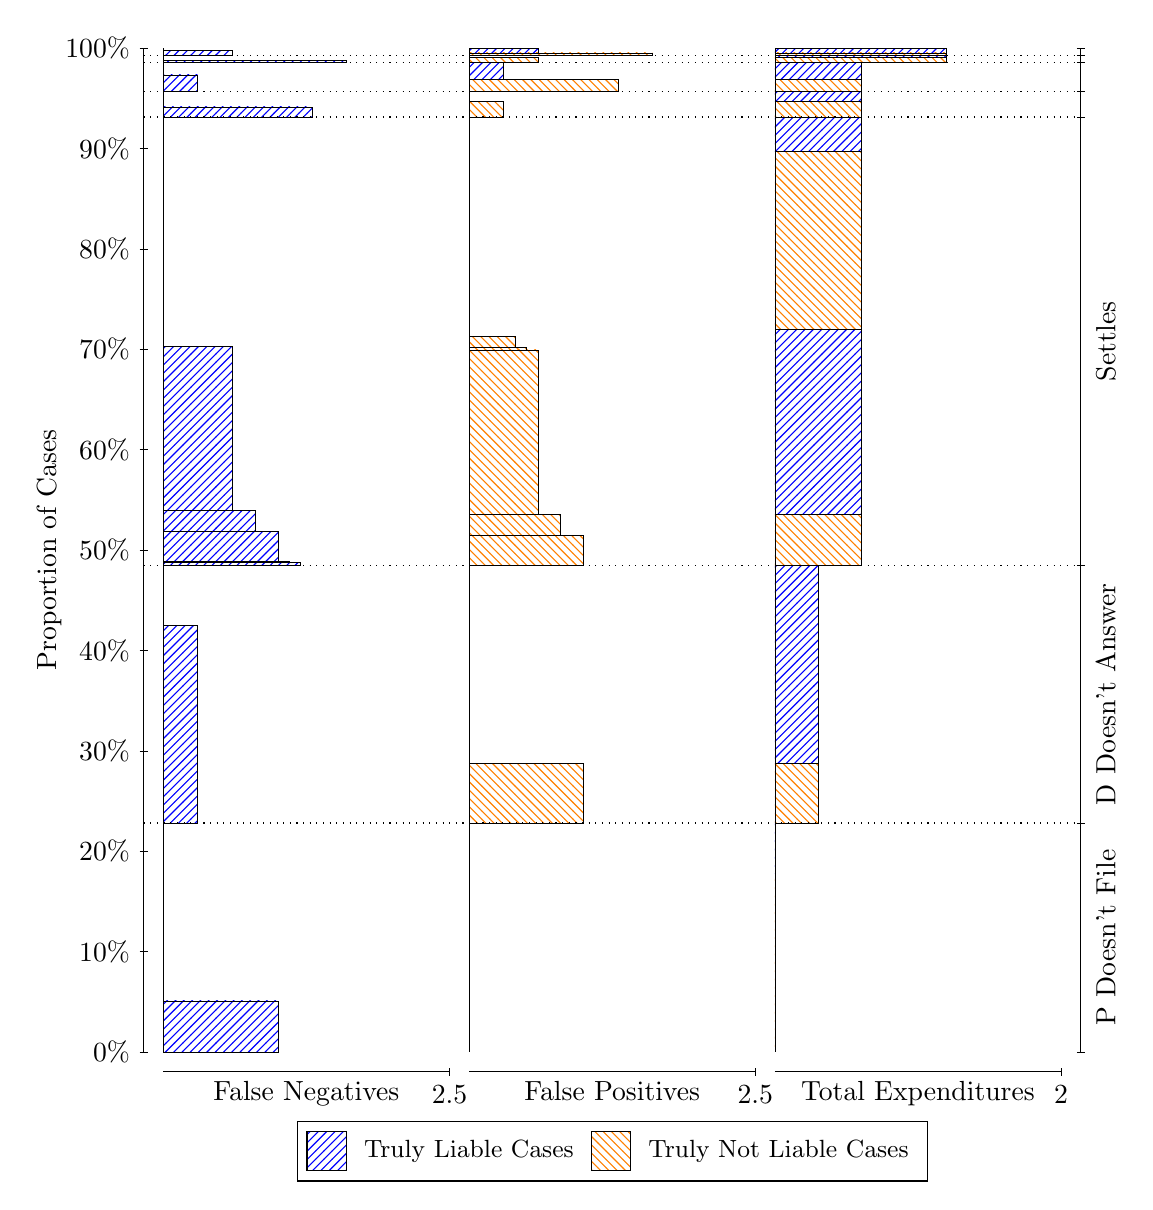
\begin{tikzpicture}
\draw[black, very thin] (1.5,1.75) -- (1.5,14.5);
\node[rotate=90, text=black, anchor=center] at (0.3, 8.125) {Proportion of Cases};
\draw[black, very thin] (1.45,1.75) -- (1.55,1.75);
\node[text=black, anchor=east] at (1.45, 1.75) {0\%};
\draw[black, very thin] (1.45,3.025) -- (1.55,3.025);
\node[text=black, anchor=east] at (1.45, 3.025) {10\%};
\draw[black, very thin] (1.45,4.3) -- (1.55,4.3);
\node[text=black, anchor=east] at (1.45, 4.3) {20\%};
\draw[black, very thin] (1.45,5.575) -- (1.55,5.575);
\node[text=black, anchor=east] at (1.45, 5.575) {30\%};
\draw[black, very thin] (1.45,6.85) -- (1.55,6.85);
\node[text=black, anchor=east] at (1.45, 6.85) {40\%};
\draw[black, very thin] (1.45,8.125) -- (1.55,8.125);
\node[text=black, anchor=east] at (1.45, 8.125) {50\%};
\draw[black, very thin] (1.45,9.4) -- (1.55,9.4);
\node[text=black, anchor=east] at (1.45, 9.4) {60\%};
\draw[black, very thin] (1.45,10.675) -- (1.55,10.675);
\node[text=black, anchor=east] at (1.45, 10.675) {70\%};
\draw[black, very thin] (1.45,11.95) -- (1.55,11.95);
\node[text=black, anchor=east] at (1.45, 11.95) {80\%};
\draw[black, very thin] (1.45,13.225) -- (1.55,13.225);
\node[text=black, anchor=east] at (1.45, 13.225) {90\%};
\draw[black, very thin] (1.45,14.5) -- (1.55,14.5);
\node[text=black, anchor=east] at (1.45, 14.5) {100\%};

\draw[black, very thin] (13.4,1.75) -- (13.4,14.5);
\draw[black, very thin] (13.35,1.75) -- (13.45,1.75);
\node[anchor=west] at (13.35, 1.75) {};
\draw[black, very thin] (13.35,4.6584) -- (13.45,4.6584);
\node[anchor=west] at (13.35, 4.6584) {};
\draw[black, very thin] (13.35,7.9307) -- (13.45,7.9307);
\node[anchor=west] at (13.35, 7.9307) {};
\draw[black, very thin] (13.35,13.624) -- (13.45,13.624);
\node[anchor=west] at (13.35, 13.624) {};
\draw[black, very thin] (13.35,13.949) -- (13.45,13.949);
\node[anchor=west] at (13.35, 13.949) {};
\draw[black, very thin] (13.35,14.313) -- (13.45,14.313);
\node[anchor=west] at (13.35, 14.313) {};
\draw[black, very thin] (13.35,14.409) -- (13.45,14.409);
\node[anchor=west] at (13.35, 14.409) {};
\draw[black, very thin] (13.35,14.5) -- (13.45,14.5);
\node[anchor=west] at (13.35, 14.5) {};

\draw[black, very thin, pattern color=blue, pattern=north east lines] (1.75,1.75) rectangle (3.2033,2.3975);
\draw[black, very thin, pattern color=orange, pattern=north west lines] (1.75,2.3975) rectangle (1.75,4.6584);
\draw[black, very thin, pattern color=blue, pattern=north east lines] (1.75,4.6584) rectangle (2.186,7.1696);
\draw[black, very thin, pattern color=orange, pattern=north west lines] (1.75,7.1696) rectangle (1.75,7.9307);
\draw[black, very thin, pattern color=blue, pattern=north east lines] (1.75,7.9307) rectangle (3.494,7.9688);
\draw[black, very thin, pattern color=blue, pattern=north east lines] (1.75,7.9688) rectangle (3.3487,7.9807);
\draw[black, very thin, pattern color=blue, pattern=north east lines] (1.75,7.9807) rectangle (3.2033,8.3652);
\draw[black, very thin, pattern color=blue, pattern=north east lines] (1.75,8.3652) rectangle (2.9127,8.6294);
\draw[black, very thin, pattern color=blue, pattern=north east lines] (1.75,8.6294) rectangle (2.622,10.715);
\draw[black, very thin, pattern color=orange, pattern=north west lines] (1.75,10.715) rectangle (1.75,13.624);
\draw[black, very thin, pattern color=blue, pattern=north east lines] (1.75,13.624) rectangle (3.6393,13.753);
\draw[black, very thin, pattern color=orange, pattern=north west lines] (1.75,13.753) rectangle (1.75,13.949);
\draw[black, very thin, pattern color=blue, pattern=north east lines] (1.75,13.949) rectangle (2.186,14.16);
\draw[black, very thin, pattern color=orange, pattern=north west lines] (1.75,14.16) rectangle (1.75,14.313);
\draw[black, very thin, pattern color=blue, pattern=north east lines] (1.75,14.313) rectangle (4.0753,14.342);
\draw[black, very thin, pattern color=orange, pattern=north west lines] (1.75,14.342) rectangle (1.75,14.409);
\draw[black, very thin, pattern color=blue, pattern=north east lines] (1.75,14.409) rectangle (2.622,14.471);
\draw[black, very thin, pattern color=orange, pattern=north west lines] (1.75,14.471) rectangle (1.75,14.5);
\draw[black, very thin, pattern color=orange, pattern=north west lines] (5.6333,1.75) rectangle (5.6333,4.0109);
\draw[black, very thin, pattern color=blue, pattern=north east lines] (5.6333,4.0109) rectangle (5.6333,4.6584);
\draw[black, very thin, pattern color=orange, pattern=north west lines] (5.6333,4.6584) rectangle (7.0867,5.4194);
\draw[black, very thin, pattern color=blue, pattern=north east lines] (5.6333,5.4194) rectangle (5.6333,7.9307);
\draw[black, very thin, pattern color=orange, pattern=north west lines] (5.6333,7.9307) rectangle (7.0867,8.3135);
\draw[black, very thin, pattern color=orange, pattern=north west lines] (5.6333,8.3135) rectangle (6.796,8.5777);
\draw[black, very thin, pattern color=orange, pattern=north west lines] (5.6333,8.5777) rectangle (6.5053,10.667);
\draw[black, very thin, pattern color=orange, pattern=north west lines] (5.6333,10.667) rectangle (6.36,10.701);
\draw[black, very thin, pattern color=orange, pattern=north west lines] (5.6333,10.701) rectangle (6.2147,10.84);
\draw[black, very thin, pattern color=blue, pattern=north east lines] (5.6333,10.84) rectangle (5.6333,13.624);
\draw[black, very thin, pattern color=orange, pattern=north west lines] (5.6333,13.624) rectangle (6.0693,13.819);
\draw[black, very thin, pattern color=blue, pattern=north east lines] (5.6333,13.819) rectangle (5.6333,13.949);
\draw[black, very thin, pattern color=orange, pattern=north west lines] (5.6333,13.949) rectangle (7.5227,14.101);
\draw[black, very thin, pattern color=blue, pattern=north east lines] (5.6333,14.101) rectangle (6.0693,14.313);
\draw[black, very thin, pattern color=orange, pattern=north west lines] (5.6333,14.313) rectangle (6.5053,14.38);
\draw[black, very thin, pattern color=blue, pattern=north east lines] (5.6333,14.38) rectangle (5.6333,14.409);
\draw[black, very thin, pattern color=orange, pattern=north west lines] (5.6333,14.409) rectangle (7.9587,14.438);
\draw[black, very thin, pattern color=blue, pattern=north east lines] (5.6333,14.438) rectangle (6.5053,14.5);
\draw[black, very thin, pattern color=orange, pattern=north west lines] (9.5167,1.75) rectangle (9.5167,4.0109);
\draw[black, very thin, pattern color=blue, pattern=north east lines] (9.5167,4.0109) rectangle (9.5167,4.6584);
\draw[black, very thin, pattern color=orange, pattern=north west lines] (9.5167,4.6584) rectangle (10.062,5.4194);
\draw[black, very thin, pattern color=blue, pattern=north east lines] (9.5167,5.4194) rectangle (10.062,7.9307);
\draw[black, very thin, pattern color=orange, pattern=north west lines] (9.5167,7.9307) rectangle (10.607,8.5777);
\draw[black, very thin, pattern color=blue, pattern=north east lines] (9.5167,8.5777) rectangle (10.607,10.928);
\draw[black, very thin, pattern color=orange, pattern=north west lines] (9.5167,10.928) rectangle (10.607,13.19);
\draw[black, very thin, pattern color=blue, pattern=north east lines] (9.5167,13.19) rectangle (10.607,13.624);
\draw[black, very thin, pattern color=orange, pattern=north west lines] (9.5167,13.624) rectangle (10.607,13.819);
\draw[black, very thin, pattern color=blue, pattern=north east lines] (9.5167,13.819) rectangle (10.607,13.949);
\draw[black, very thin, pattern color=orange, pattern=north west lines] (9.5167,13.949) rectangle (10.607,14.101);
\draw[black, very thin, pattern color=blue, pattern=north east lines] (9.5167,14.101) rectangle (10.607,14.313);
\draw[black, very thin, pattern color=orange, pattern=north west lines] (9.5167,14.313) rectangle (11.697,14.38);
\draw[black, very thin, pattern color=blue, pattern=north east lines] (9.5167,14.38) rectangle (11.697,14.409);
\draw[black, very thin, pattern color=orange, pattern=north west lines] (9.5167,14.409) rectangle (11.697,14.438);
\draw[black, very thin, pattern color=blue, pattern=north east lines] (9.5167,14.438) rectangle (11.697,14.5);
\draw[black, dotted] (1.5,4.6584) -- (13.4,4.6584);
\draw[black, dotted] (1.5,7.9307) -- (13.4,7.9307);
\draw[black, dotted] (1.5,13.624) -- (13.4,13.624);
\draw[black, dotted] (1.5,13.949) -- (13.4,13.949);
\draw[black, dotted] (1.5,14.313) -- (13.4,14.313);
\draw[black, dotted] (1.5,14.409) -- (13.4,14.409);
\draw[black, very thin] (1.75,1.5) -- (5.3833,1.5);
\node[text=black, anchor=north] at (3.5667, 1.5) {False Negatives};
\draw[black, very thin] (5.3833,1.45) -- (5.3833,1.55);
\node[text=black, anchor=north] at (5.3833, 1.45) {2.5};

\draw[black, very thin] (5.6333,1.5) -- (9.2667,1.5);
\node[text=black, anchor=north] at (7.45, 1.5) {False Positives};
\draw[black, very thin] (9.2667,1.45) -- (9.2667,1.55);
\node[text=black, anchor=north] at (9.2667, 1.45) {2.5};

\draw[black, very thin] (9.5167,1.5) -- (13.15,1.5);
\node[text=black, anchor=north] at (11.333, 1.5) {Total Expenditures};
\draw[black, very thin] (13.15,1.45) -- (13.15,1.55);
\node[text=black, anchor=north] at (13.15, 1.45) {2};

\node[text=black, centered, rotate=90] at (13.72, 3.2042) {P Doesn't File};
\node[text=black, centered, rotate=90] at (13.72, 6.2945) {D Doesn't Answer};
\node[text=black, centered, rotate=90] at (13.72, 10.777) {Settles};





\draw (7.449999999999999,1.5) node[draw=none] (baseCoordinate) {};
\begin{scope}[align=center]
        \matrix[scale=0.5, draw=black, below=0.5cm of baseCoordinate, nodes={draw}, column sep=0.1cm]{
            \node[rectangle, draw, minimum width=0.5cm, minimum height=0.5cm, pattern color=blue, pattern=north east lines] {}; &
            \node[draw=none, font=\small, text=black] (B) {Truly Liable Cases}; &
            \node[rectangle, draw, minimum width=0.5cm, minimum height=0.5cm, pattern color=orange, pattern=north west lines] {}; &
            \node[draw=none, font=\small, text=black] (B) {Truly Not Liable Cases}; \\
            };
\end{scope}

\end{tikzpicture}
\end{document}